\documentclass[]{article}
\usepackage{lmodern}
\usepackage{amssymb,amsmath}
\usepackage{ifxetex,ifluatex}
\usepackage{fixltx2e} % provides \textsubscript
\ifnum 0\ifxetex 1\fi\ifluatex 1\fi=0 % if pdftex
  \usepackage[T1]{fontenc}
  \usepackage[utf8]{inputenc}
\else % if luatex or xelatex
  \ifxetex
    \usepackage{mathspec}
  \else
    \usepackage{fontspec}
  \fi
  \defaultfontfeatures{Ligatures=TeX,Scale=MatchLowercase}
\fi
% use upquote if available, for straight quotes in verbatim environments
\IfFileExists{upquote.sty}{\usepackage{upquote}}{}
% use microtype if available
\IfFileExists{microtype.sty}{%
\usepackage{microtype}
\UseMicrotypeSet[protrusion]{basicmath} % disable protrusion for tt fonts
}{}
\usepackage[margin=1in]{geometry}
\usepackage{hyperref}
\hypersetup{unicode=true,
            pdftitle={Assignment 5},
            pdfauthor={Alex Ivina},
            pdfborder={0 0 0},
            breaklinks=true}
\urlstyle{same}  % don't use monospace font for urls
\usepackage{graphicx,grffile}
\makeatletter
\def\maxwidth{\ifdim\Gin@nat@width>\linewidth\linewidth\else\Gin@nat@width\fi}
\def\maxheight{\ifdim\Gin@nat@height>\textheight\textheight\else\Gin@nat@height\fi}
\makeatother
% Scale images if necessary, so that they will not overflow the page
% margins by default, and it is still possible to overwrite the defaults
% using explicit options in \includegraphics[width, height, ...]{}
\setkeys{Gin}{width=\maxwidth,height=\maxheight,keepaspectratio}
\IfFileExists{parskip.sty}{%
\usepackage{parskip}
}{% else
\setlength{\parindent}{0pt}
\setlength{\parskip}{6pt plus 2pt minus 1pt}
}
\setlength{\emergencystretch}{3em}  % prevent overfull lines
\providecommand{\tightlist}{%
  \setlength{\itemsep}{0pt}\setlength{\parskip}{0pt}}
\setcounter{secnumdepth}{0}
% Redefines (sub)paragraphs to behave more like sections
\ifx\paragraph\undefined\else
\let\oldparagraph\paragraph
\renewcommand{\paragraph}[1]{\oldparagraph{#1}\mbox{}}
\fi
\ifx\subparagraph\undefined\else
\let\oldsubparagraph\subparagraph
\renewcommand{\subparagraph}[1]{\oldsubparagraph{#1}\mbox{}}
\fi

%%% Use protect on footnotes to avoid problems with footnotes in titles
\let\rmarkdownfootnote\footnote%
\def\footnote{\protect\rmarkdownfootnote}

%%% Change title format to be more compact
\usepackage{titling}

% Create subtitle command for use in maketitle
\newcommand{\subtitle}[1]{
  \posttitle{
    \begin{center}\large#1\end{center}
    }
}

\setlength{\droptitle}{-2em}

  \title{Assignment 5}
    \pretitle{\vspace{\droptitle}\centering\huge}
  \posttitle{\par}
    \author{Alex Ivina}
    \preauthor{\centering\large\emph}
  \postauthor{\par}
      \predate{\centering\large\emph}
  \postdate{\par}
    \date{November 26, 2018}

\usepackage{booktabs}
\usepackage{longtable}
\usepackage{array}
\usepackage{multirow}
\usepackage[table]{xcolor}
\usepackage{wrapfig}
\usepackage{float}
\usepackage{colortbl}
\usepackage{pdflscape}
\usepackage{tabu}
\usepackage{threeparttable}
\usepackage{threeparttablex}
\usepackage[normalem]{ulem}
\usepackage{makecell}

\begin{document}
\maketitle

\begin{enumerate}
\def\labelenumi{\arabic{enumi}.}
\tightlist
\item
  Male and female graduate enrollment (1967 - 2015). Compare trends in
  total graduate enrollment for males and females (including
  full-time/part-time and private/public universities) in the United
  States from 1967 - 2015. Describe your results statistically,
  graphically and in text.
\end{enumerate}

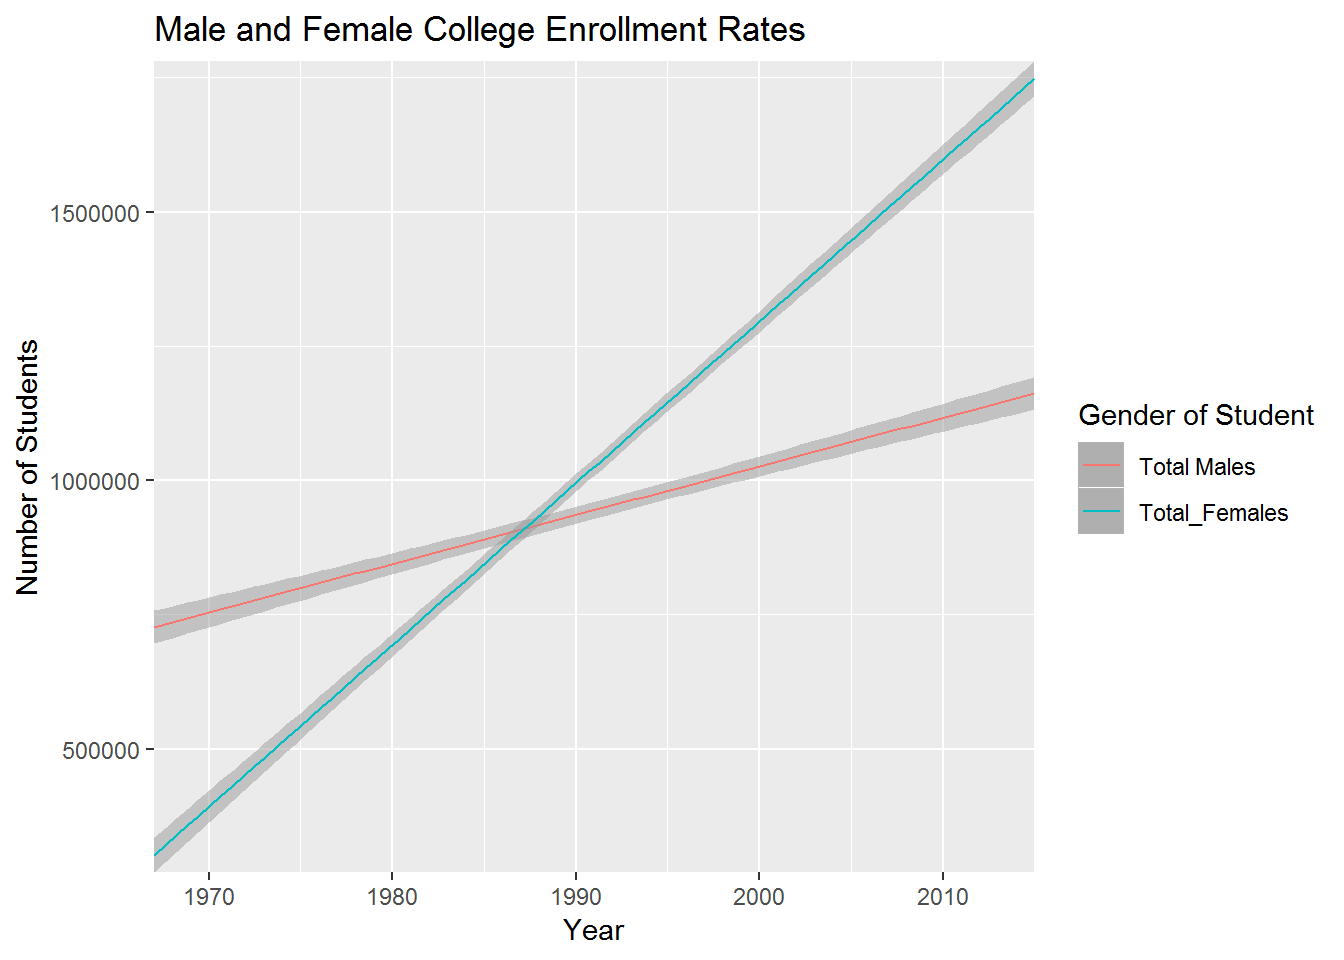
\includegraphics{Assignment_5_files/figure-latex/Model Graph-1.pdf}

Written Results: Total\_Males- Year significantly predicts college
enrollment rates for males (b = 9069, t(47) = 16.61, p \textless{}
0.001) with a strong positive correlation between the two (Pearson's r =
0.92). The overall model (Total Male enrollment = -17,112,153 + 9069
(Year) explains a significant amount of variance in enrollment rate
(F(1,47) = 476, p \textless{} 0.001, R2 = 0.8545).''

male\_enrollment = -17112153 + 9069(Year)

Total\_Females- Year significantly predicts college enrollment rates for
females (b = 30126, t(47) = 51.66, p \textless{} 0.001) with a strong
positive correlation between the two (Pearson's r = 0.99). The overall
model (Total Female enrollment = -58955502 + 30126 (Year) explains a
significant amount of variance in enrollment rate (F(1,47) = 2669, p
\textless{} 0.001, R2 = 0.9827).

female\_enrollment = -0.0000005896 + 30130(Year)

\begin{enumerate}
\def\labelenumi{\arabic{enumi}.}
\setcounter{enumi}{1}
\tightlist
\item
  Shifts in female PhD recipients by field (1985, 2000, and 2015).
  Describe if and how there was a shift in PhDs awarded to females in
  four fields (Physical and Earth Sciences, Engineering, Education, and
  Humanities \& Arts) in 1985, 2000, and 2015. Describe your results
  statistically, in a graph or table, and in text. Note: There are
  several ways that you can interpret this question. You are invited to
  decide which you think is/are most interesting. Just be really clear
  about what you are asking/answering in your report.
\end{enumerate}

\begin{verbatim}
## 
##  Pearson's Chi-squared test
## 
## data:  Phds_new
## X-squared = 2898, df = 14, p-value < 2.2e-16
\end{verbatim}

\begin{table}

\caption{\label{tab:unnamed-chunk-3}Changes in field of study }
\centering
\begin{tabular}[t]{l|r|r|r}
\hline
  & 1985 & 2000 & 2015\\
\hline
Female\_Physical\_science & 0.16 & 0.29 & 0.56\\
\hline
Female\_Engineering & 0.06 & 0.25 & 0.69\\
\hline
Female\_Education & 0.31 & 0.37 & 0.31\\
\hline
Female\_Humanities & 0.20 & 0.39 & 0.41\\
\hline
\end{tabular}
\end{table}

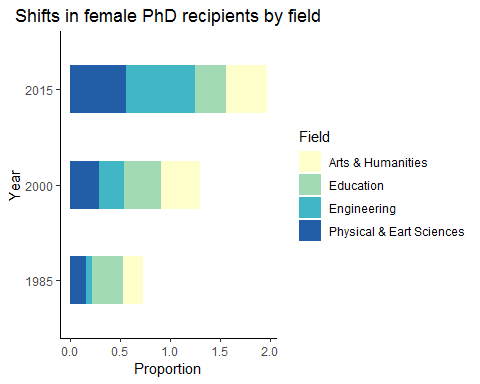
\includegraphics{Assignment_5_files/figure-latex/unnamed-chunk-3-1.pdf}

The proportion of female phD recipients increased in three fields
(Physical \& Earth Sciences, Engineering, and Arts \& Humanities) in
1985, 2000, 2015.

\begin{enumerate}
\def\labelenumi{\arabic{enumi}.}
\setcounter{enumi}{2}
\tightlist
\item
  Male and female salaries for starting postdoctoral and other
  employment positions (2015). Compare median salaries for male and
  female doctorate recipients in 2015. Answer these two questions: Does
  median salary differ significantly between male and female starting
  postdoc positions? Does median salary differ significantly between
  male and female PhD recipients in non-postdoc employment positions?
\end{enumerate}

=======

Communicating Statistical Results: Non-Parametric Wilcomxon Signed Rank
anaylsis for data collected from 15 fields of study in the year 2015
revealed that the median salaries (in dollars) differed significantly
for male and female PhD recipients in non-postdoc employment positions
(V= 101, p=0.003). In all fields except Physics \& Astonomy, men
recieved either equal or moderately higher salaries(cliffs delta=0.213).

However, a separate non-parametric wimcoxon signed rank test for PhD
recipients starting posdoc positions revealed that there was \emph{not}
a signficant difference between salaries for males and females (V=19.5,
p=.888). In several fields of study, males and females recieved the
exact same salary. Females recieved a slightly higher median salary in
some fields, while males were paid slightly more in others (cliffs
delta=.04).

\begin{enumerate}
\def\labelenumi{\arabic{enumi}.}
\setcounter{enumi}{3}
\tightlist
\item
  Exploring academic salaries for professors in U.S. colleges. Explore
  relationships between variables in the `Faculty salary data (2008 -
  2009 survey)' dataset. Develop a model describing faculty salary based
  on data for faculty sex, rank, years in current position, field, and
  number of years since doctoral degree was earned. You should make
  decisions regarding which variables should remain in your final model.
  Describe the results qualitatively and quantitatively (i.e., don't
  just report the statistical results of the model -- make sure you
  describe interesting findings in text). You can also discuss any
  concerns that you have with the model(s) you present, if any
\end{enumerate}

Dependent variable:

salary

faculty\_rankAssocProf

-32,928.400***

(3,544.403)

faculty\_rankAsstProf

-46,032.550***

(4,240.120)

years\_since\_phd

61.011

(127.010)

sexMale

4,349.366

(3,875.393)

disciplineTheoretical

-13,937.470***

(2,346.534)

Constant

127,854.300***

(5,084.988)

Observations

397

R2

0.447

Adjusted R2

0.440

Residual Std. Error

22,663.240 (df = 391)

F Statistic

63.266*** (df = 5; 391)

Note:

\emph{p\textless{}0.1; \textbf{p\textless{}0.05; }}p\textless{}0.01

Write Up:

Formula: salary = 127854.34 -32928.4(Associate\_Professor) -
46032.55(Assitant\_Professor) + 61.01(years\_since\_phd) +
4349.37(sexMale) - 13937.47(disciplineTheoretical)

The formula for faculty salary will predict salary as a function of a
professors rank (here we are using professor as the refrence level and
comparing against associate professor and assitant professor), years
since someone has gained their PHD, their sex ( here female is the
refrence level and male is included in the graph) and lastly discipline
(we only look at if the diswcipline is theoretical or applied and here
we use applied as the refrence level). What we found was that professors
were paid the most and assitant profressors the least by rank and that
years every year after your PHD you earned slightly more. It was also
apparent that males earned higher wages than femlaes and that those in
theoretical disciplines earned less than those in technical disciplines.
Over all these variables accounted for 44\% (R\textsuperscript{2} =
0.4401) of changes in salary. Looking at the variables observed the rank
of a professor and the deispline showed significant results
(p-value\textless{}0.001) where as sex and years since one earned their
PHD did not yeild significant results (p-value\textgreater{}0.001).

\begin{verbatim}
## 
## Call:
## lm(formula = salary ~ years_since_phd + years_employed + sex + 
##     discipline, data = faculty_salary1)
## 
## Coefficients:
##           (Intercept)        years_since_phd         years_employed  
##               87651.2                 1804.1                 -770.1  
##               sexMale  disciplineTheoretical  
##                7545.3               -16325.4
\end{verbatim}

\begin{verbatim}
## 
## Call:
## lm(formula = salary ~ years_since_phd + years_employed + sex + 
##     discipline, data = faculty_salary1)
## 
## Residuals:
##    Min     1Q Median     3Q    Max 
## -75974 -17094  -3799  16073  97055 
## 
## Coefficients:
##                       Estimate Std. Error t value Pr(>|t|)    
## (Intercept)            87651.2     4666.2  18.784  < 2e-16 ***
## years_since_phd         1804.1      248.9   7.249 2.25e-12 ***
## years_employed          -770.1      244.1  -3.155  0.00173 ** 
## sexMale                 7545.3     4462.6   1.691  0.09167 .  
## disciplineTheoretical -16325.4     2708.9  -6.027 3.87e-09 ***
## ---
## Signif. codes:  0 '***' 0.001 '**' 0.01 '*' 0.05 '.' 0.1 ' ' 1
## 
## Residual standard error: 26130 on 392 degrees of freedom
## Multiple R-squared:  0.2634, Adjusted R-squared:  0.2558 
## F-statistic: 35.04 on 4 and 392 DF,  p-value: < 2.2e-16
\end{verbatim}

\begin{verbatim}
## 
## Call:
## lm(formula = salary ~ years_since_phd + years_employed + sex + 
##     discipline + years_since_phd * years_employed, data = faculty_salary1)
## 
## Coefficients:
##                    (Intercept)                 years_since_phd  
##                       67764.10                         2391.08  
##                 years_employed                         sexMale  
##                        1473.92                         8188.37  
##          disciplineTheoretical  years_since_phd:years_employed  
##                      -14999.33                          -62.23
\end{verbatim}

\begin{verbatim}
## 
## Call:
## lm(formula = salary ~ years_since_phd + years_employed + sex + 
##     discipline + years_since_phd * years_employed, data = faculty_salary1)
## 
## Residuals:
##    Min     1Q Median     3Q    Max 
## -55902 -14672  -1759  12687  98576 
## 
## Coefficients:
##                                  Estimate Std. Error t value Pr(>|t|)    
## (Intercept)                     67764.105   4849.353  13.974  < 2e-16 ***
## years_since_phd                  2391.078    237.860  10.052  < 2e-16 ***
## years_employed                   1473.923    341.469   4.316 2.01e-05 ***
## sexMale                          8188.367   4090.693   2.002    0.046 *  
## disciplineTheoretical          -14999.332   2487.418  -6.030 3.80e-09 ***
## years_since_phd:years_employed    -62.226      7.153  -8.699  < 2e-16 ***
## ---
## Signif. codes:  0 '***' 0.001 '**' 0.01 '*' 0.05 '.' 0.1 ' ' 1
## 
## Residual standard error: 23950 on 391 degrees of freedom
## Multiple R-squared:  0.3828, Adjusted R-squared:  0.3749 
## F-statistic:  48.5 on 5 and 391 DF,  p-value: < 2.2e-16
\end{verbatim}

\begin{verbatim}
##                years_since_phd                 years_employed 
##                       6.488255                      13.619794 
##                            sex                     discipline 
##                       1.026208                       1.062488 
## years_since_phd:years_employed 
##                      13.062127
\end{verbatim}

\begin{verbatim}
## [1] 9140.98
\end{verbatim}

Dependent variable:

salary

years\_since\_phd

2,391.078***

(237.860)

years\_employed

1,473.923***

(341.469)

sexMale

8,188.367**

(4,090.693)

disciplineTheoretical

-14,999.330***

(2,487.418)

years\_since\_phd:years\_employed

-62.226***

(7.153)

Constant

67,764.100***

(4,849.353)

Observations

397

R2

0.383

Adjusted R2

0.375

Residual Std. Error

23,947.360 (df = 391)

F Statistic

48.501*** (df = 5; 391)

Note:

\emph{p\textless{}0.1; \textbf{p\textless{}0.05; }}p\textless{}0.01

Model: \$67,764.10+ \$2391.08(years since phd)+
\$1473.92(years\_employed)+
\$8188.37(sexMale)-\$14999.33(disciplineTheoretical)
-62.23(years\_since\_phd:years\_employed)

According to the model, professors expect: -base pay of \$67,764.10
-Additional \$2,391 for each year since phd -Additional \$1,473 for each
successive year employed -Males to earn \$8,188 more per year than
females -Professors in the theoretical disciplines to earn about
\$15,000 less per year than professors in the applied disiplines.

Each of these factors is statistically significant (years\_since\_phd,
p=\textless{}.001, years\_employed, p=\textless{}.001, sexMale P=0.046,
disciplineTheoretical p=\textless{}.001). Overall model significantly
predicts outcomes (p\textless{}.001).


\end{document}
